% Diagrama 4: Flujo experimental y de análisis (Parte 4)
% Compilar con: lualatex flujo-experimental.tex  (sale flujo-experimental.pdf)
\documentclass[tikz,border=16pt]{standalone}
\usetikzlibrary{positioning,arrows.meta}
\usepackage{amsmath}
\begin{document}
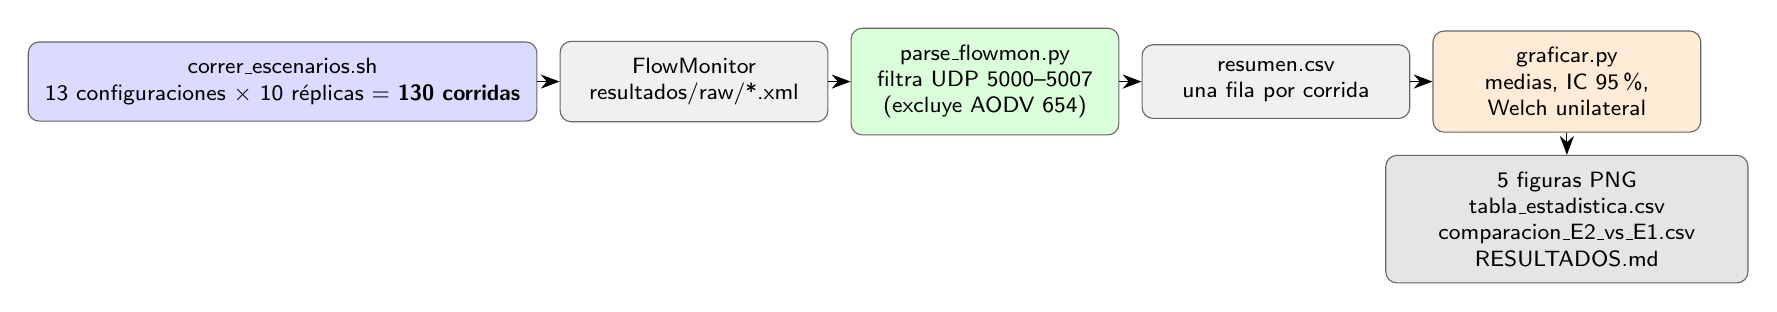
\begin{tikzpicture}[
  font=\sffamily\footnotesize,
  box/.style={draw=black!60, rounded corners=4pt, align=center,
              minimum width=3.4cm, inner sep=6pt, fill=#1},
  arr/.style={-{Stealth[length=2.4mm]}},
]
\node[box=blue!14] (correr) {correr\_escenarios.sh\\ 13 configuraciones $\times$ 10 réplicas = \textbf{130 corridas}};
\node[box=black!6] (xml) [right=8pt of correr] {FlowMonitor\\ resultados/raw/*.xml};
\node[box=green!14] (parse) [right=8pt of xml] {parse\_flowmon.py\\ filtra UDP 5000--5007\\(excluye AODV 654)};
\node[box=black!6] (csv) [right=8pt of parse] {resumen.csv\\ una fila por corrida};
\node[box=orange!16] (graf) [right=8pt of csv] {graficar.py\\ medias, IC 95\,\%,\\ Welch unilateral};
\node[box=black!10] (out) [below=8pt of graf, minimum width=4.6cm] {5 figuras PNG\\ tabla\_estadistica.csv\\ comparacion\_E2\_vs\_E1.csv\\ RESULTADOS.md};

\draw[arr] (correr) -- (xml);
\draw[arr] (xml) -- (parse);
\draw[arr] (parse) -- (csv);
\draw[arr] (csv) -- (graf);
\draw[arr] (graf) -- (out);
\end{tikzpicture}
\end{document}
